\section{Experimental Results}
\label{sec:result}

We simulate the behavior of the proposed ML-resistant PUF using Python. The statistics of raw SRAM PUF responses are based on \cite{maes2013accurate, maes2009soft}. The logical behavior of other digital circuits are accurately captured by software. We virtually manufacture (simulate) $1000$ distinct lattice PUF instances with design parameters chosen in Section \ref{sec:design}. The CRPs of the PUF instances are collected to examine: (1) statistical characteristics (uniformity, uniqueness, and reliability), and (2) resistance to leading ML modeling attacks. The whole lattice PUF design (besides the SRAM PUF) is implemented on a Xilinx Spartan-6 FPGA.


\subsection{Statistical Analysis}
\label{sec:statistical_result}
%\textbf{Uniformity} of a PUF characterizes unbiasedness, namely, the proportion of `0's and `1's in the output responses.
%For an ideal PUF $f$, the proportion needs to be $50\%$ for either `0' or `1'.
%Uniformity is formally defined as the average Hamming weight $\HW(f)$ of responses $\mathbf{r}$ over randomly sampled challenges $\mathbf{c}$'s \cite{maiti2013systematic}:
%\begin{equation*}
%\HW(f)= \Expect_\mathbf{c}[\HW(\mathbf{r})] = \Expect_{\mathbf{c}}[\HW(f(\mathbf{c}))].
%\end{equation*}
%Here $\Expect_X$ represents expectation over random variable $X$.
%Note that $\mathbf{c}$ follows the ciphertext distribution rather than the usual uniform distribution \cite{maiti2013systematic}.
%Figure \ref{fig:HW} shows uniformity obtained using $1000$ randomly selected challenges. 
%The distribution is centered at $49.98\%$, the standard deviation is $1.58\%$. 


%\textbf{Uniqueness} measures the ability of a PUF to be uniquely distinguished among a set of PUFs. 
%Based on \cite{maiti2013systematic}, we define this metric to be the average inter-class HD of responses $(\mathbf{r}_i,\mathbf{r}_j)$ under the same challenges $\mathbf{c}$ for a randomly picked PUF pair $(f_i, f_j)$:
%\begin{equation*}
%\HD(f_i,f_j) = \Expect_\mathbf{c}[\HD(\mathbf{r}_i,\mathbf{r}_j)]=\Expect_{\mathbf{c}}[\HD(f_i(\mathbf{c}),f_j(\mathbf{c}))].
%\end{equation*}
%For ideal PUFs, responses under the same challenges are orthogonal, namely, $\HD(f_i,f_j)$'s are close to $50\%$.
%Uniqueness is also evaluated under the ciphertext distribution.  

%Uniqueness is shown in Figure \ref{fig:inter_intra}, evaluated for $1000$ PUF instances. 
%The lattice PUF achieves near-optimal uniqueness: inter-class HD is centered at $50.00\%$, its standard deviation is $1.58\%$. 

%\textbf{Reliability} of a PUF $f$ is characterized by the average BER of outputs with respect to their enrollment values:
%\begin{equation*}
%\BER = \Expect_{f^\prime}[\HD(f,f^\prime)]= \Expect_{f^\prime,\mathbf{c}}[\HD(f(\mathbf{c}),f^\prime(\mathbf{c}))].
%\end{equation*}
%As discussed in Section \ref{sec:design}, the overall BER of the lattice PUF is due to two components: the failure rate of key reconstruction and LWE decryption error rate.
%Intra-class HD in Figure \ref{fig:inter_intra} reflects the result of decryption errors by assuming a perfect key reconstruction. 

In this section, we examine statistical metrics of the proposed PUF. Uniformity, uniqueness and reliability are commonly adopted metrics to evaluate the statistical performance of a PUF \cite{maiti2013systematic}. \textbf{Uniformity} measures the mean Hamming Weight of responses from a PUF under a set of random challenges. The ideal uniformity is 0.5, which indicates the zero bits and the one bits are distributed uniformly in PUF response. \textbf{Uniqueness} measures the mean Hamming Distance of PUF responses between a pair of different PUF instances (inter-class HD), with the same set of PUF challenges. The ideal uniqueness is 0.5, which means each PUF instance produces a unique response distribution. \textbf{Reliability} measures the mean Hamming Distance between actual PUF responses and the enrolled (ideal) PUF responses (intra-class HD). The ideal PUF is expected to have no bit flips in responses compared to the enrolled values.

We evaluate the metrics with 1000 lattice PUF instances and 1000 random challenges following LWE ciphertext distribution \cite{maiti2013systematic}. The lattice PUF demonstrates near ideal statistical properties: the mean of uniformity distribution is 0.4998 (std = 0.0158) and the mean of uniqueness distribution is 0.5 (std = 0.0158). To evaluate PUF reliability, we assume the key reconstruction process is ideal and the errors merely come from LWE decryption. Figure \ref{fig:inter_intra} shows the lattice PUF reliability distribution centers close to 0. 



%\begin{figure}[t!]
%\centering
%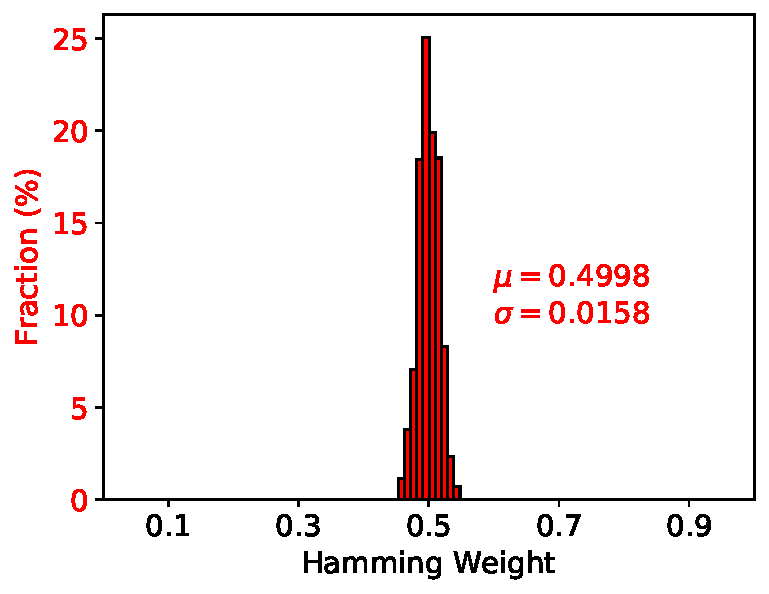
\includegraphics[width = 0.7\linewidth]{./figs/HW.pdf}
%\caption{Uniformity of lattice PUF output.}
%\label{fig:HW}
%\end{figure}

%\begin{figure}[t!]
%\centering
%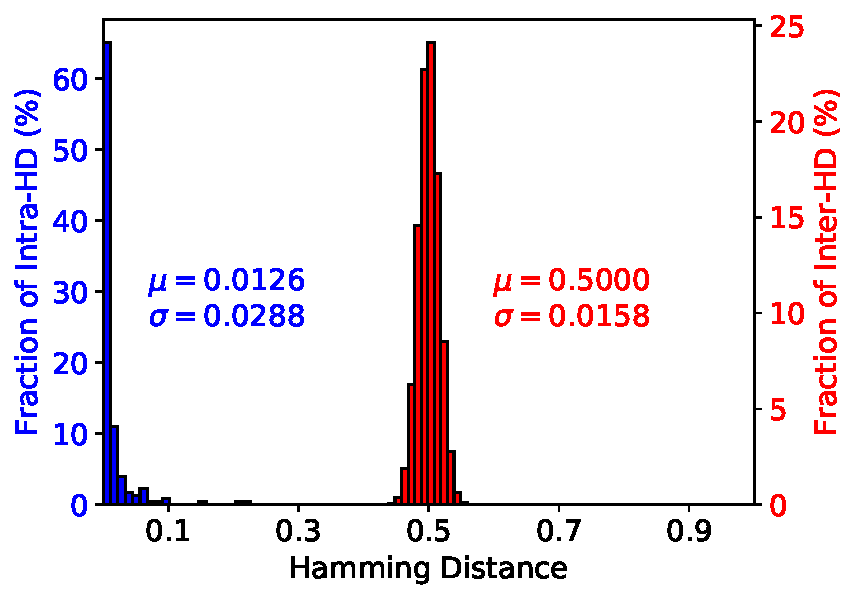
\includegraphics[width = 0.75\linewidth]{./figs/inter_intra.pdf}
%\caption{Uniqueness and reliability of lattice PUF output.}
%\label{fig:inter_intra}
%\end{figure}

\begin{figure} 
    \centering
  \subfloat[\label{fig:HW}]{%
       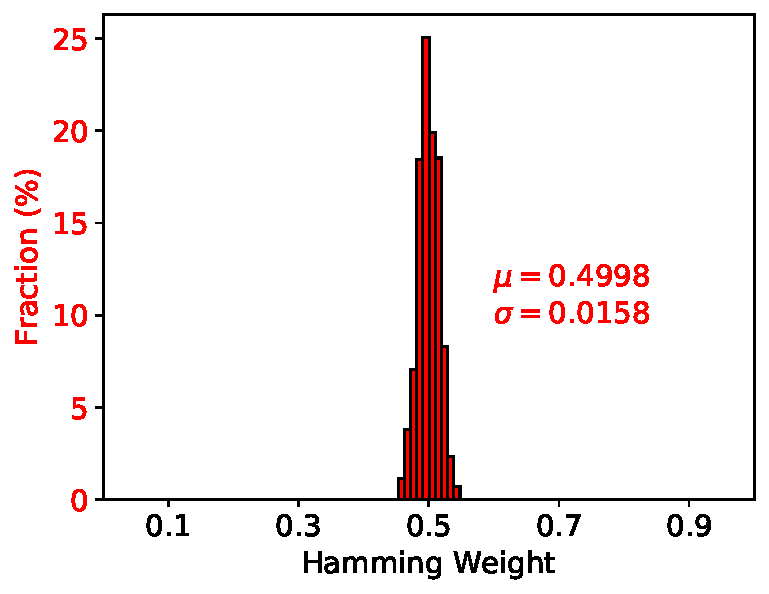
\includegraphics[width=0.45\linewidth]{./figs/HW.pdf}}
    \hfill
  \subfloat[\label{fig:inter_intra}]{%
        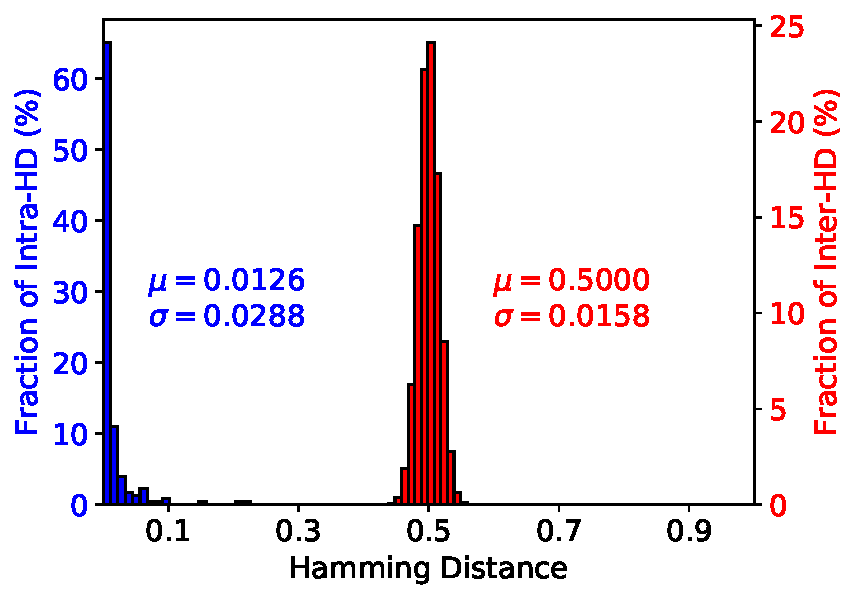
\includegraphics[width=0.5\linewidth]{./figs/inter_intra.pdf}}
  \caption{(a) Lattice PUF has near ideal uniformity. (b) Lattice PUF has near ideal uniqueness and reliability.}
  \label{fig: lattice_puf_stats} 
\end{figure}

%\begin{figure}[t!]
%\centering
%\begin{subfigure}{0.2\textwidth}
%   \centering
%   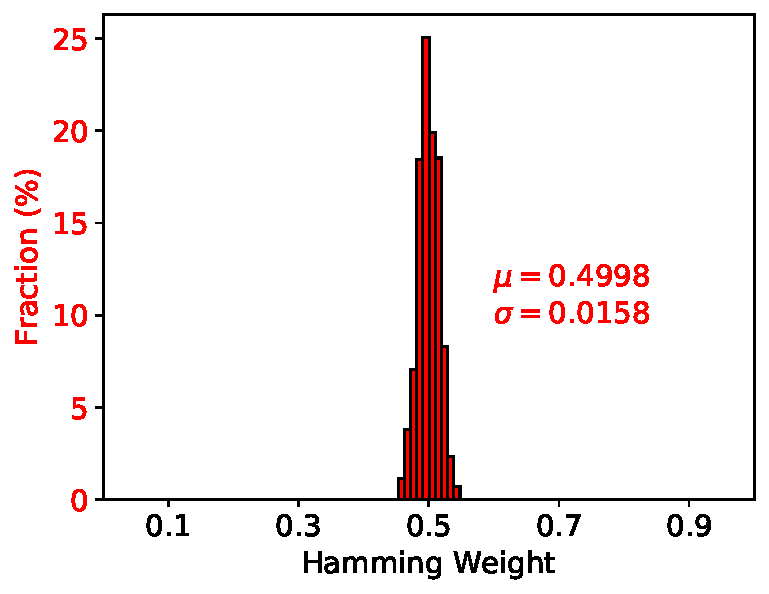
\includegraphics[width=\textwidth]{./figs/HW.pdf}
   %\caption{Uniformity of lattice PUF output.}
%   \label{fig:HW} 
%\end{subfigure}
%\begin{subfigure}{0.24\textwidth}
%   \centering
%   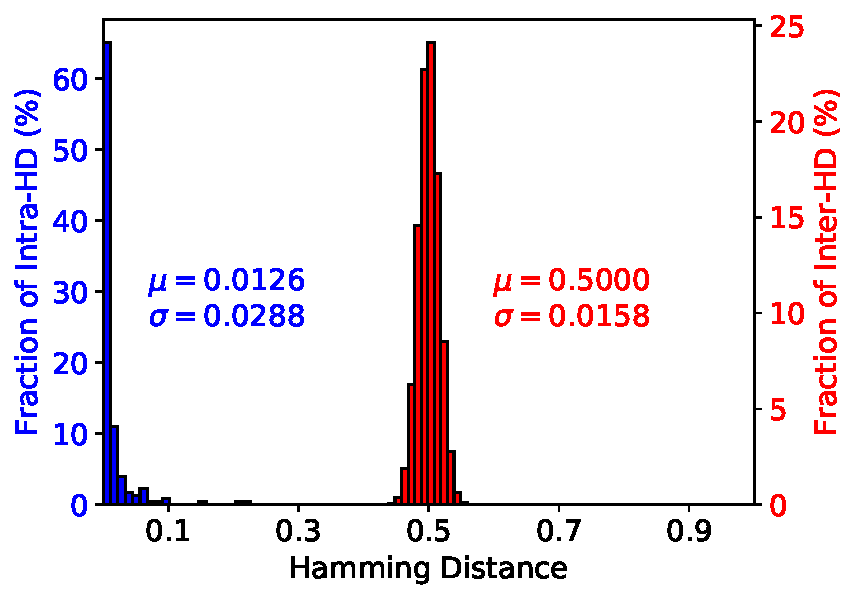
\includegraphics[width=\textwidth]{./figs/inter_intra.pdf}
   %\caption{Uniqueness and reliability of lattice PUF output.}
%   \label{fig:inter_intra}
%\end{subfigure}
%\caption{(a) Uniformity of lattice PUF output. (b) Uniqueness and reliability of lattice PUF output.}
%\label{power_trace_avg_untrusted_devices_1_to_15}
%\end{figure}

\subsection{ML Attacks on Lattice PUF}

%While the ultimate promise of lattice PUF is due to its theoretically-supported reliance on hard computational problems,
%testing its ML resistance empirically gives a concrete measure of its security. The resistance of lattice PUF is evaluated with a series of traditional (i.e., not based on deep learning) ML algorithms, including SVM, LR, and single-layer NN (1-NN), as well as a number of DNNs.
%We use the Python scikit-learn %\cite{scikit-learn} 
%package to implement SVM and LR.  
%The SVM uses the radial basis function (RBF) kernel.
%The 1-NN model uses only one hidden feed-forward layer composed of 100 neurons, with the rectified linear unit (ReLU) as the activation function. 
%Training of 1-NNs and subsequent DNNs are implemented using Keras %\cite{chollet2015keras} 
%with TensorFlow %\cite{abadi2016tensorflow} 
%backend.

Although we establish the security of lattice PUF theoretically, we perform empirical validation as a way to explore the possible attacks of distributional relaxations used, and as a way to give added overall confidence in the design. The traditional ML algorithms include LR, SVM and one-layer Neural Network (1-NN). The LR and SVM are implemented with scikit-learn package in Python. We use the RBF kernel in SVM, which models a non-linear decision boundary. The single hidden layer of 1-NN consists of 100 neurons, and the activation function is selected to be ReLU. We train the 1-NN and DNNs with Keras powered by Tensorflow.


\begin{figure}[t!]
\centering
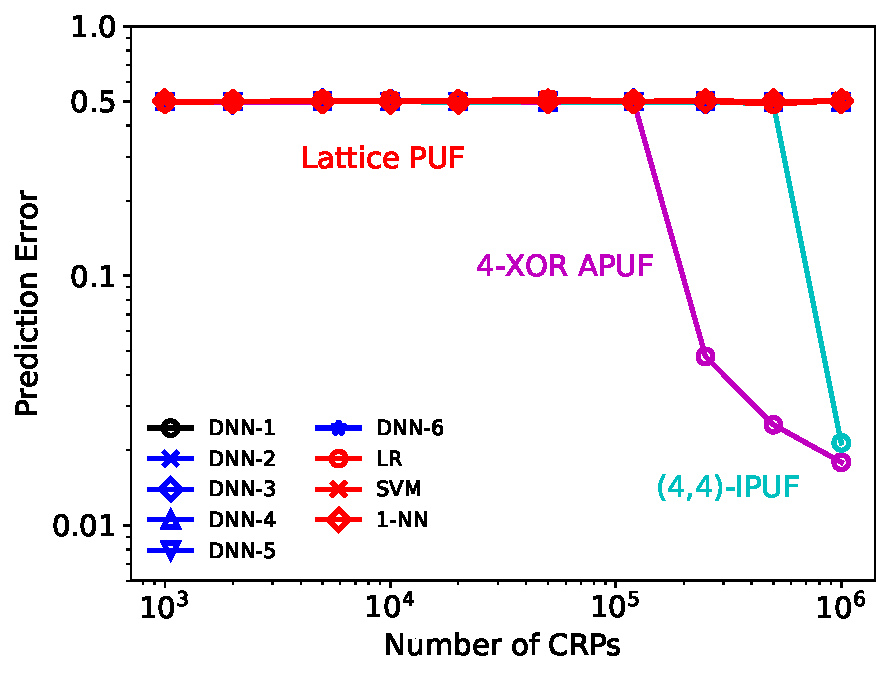
\includegraphics[width = 0.7\linewidth]{./figs/ml_attack_dnn_all_puf_5_new.pdf}
\caption{Lattice PUF is resilient to multiple ML modeling attacks including DNNs. Two other strong PUFs are ultimately vulnerable to DNN-based attacks.}
\label{fig:ml_attack_2}
\end{figure}

\begin{figure}[t!]
\centering
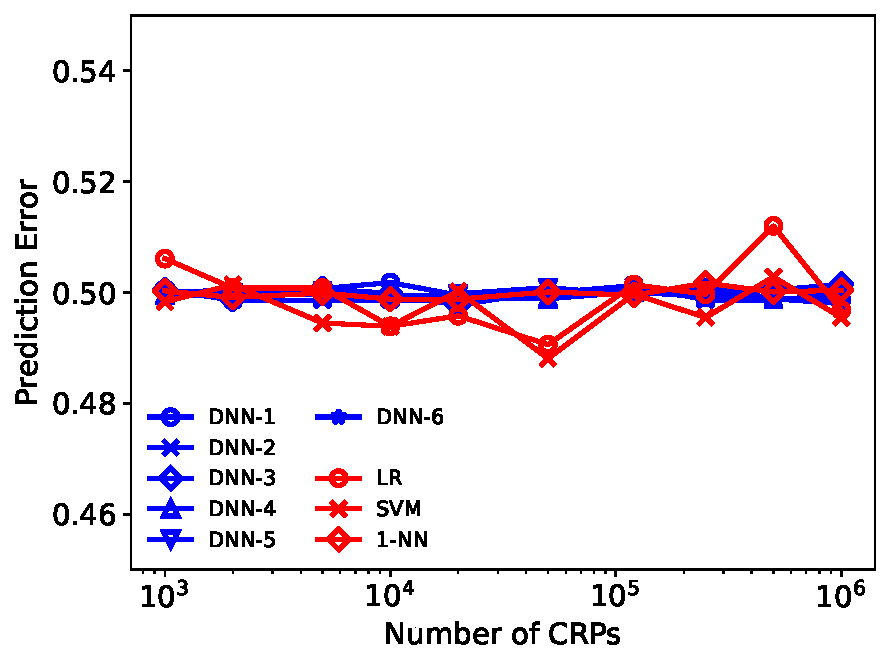
\includegraphics[width = 0.7\linewidth]{./figs/ml_attack_lattice_puf_new.pdf}
\caption{Lattice PUF can not be broken by both conventional ML algorithms and more powerful DNNs.}
\label{fig:ml_attack_3}
\end{figure}

%\begin{figure}[t!] 
%    \centering
%  \subfloat[\label{fig:ml_attack_2}]{%
%       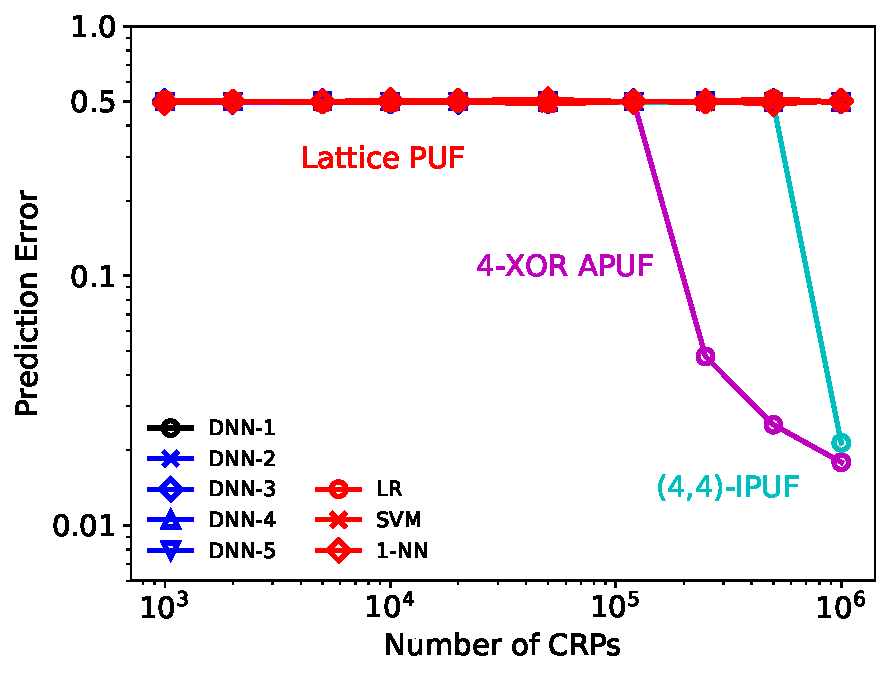
\includegraphics[width=0.5\linewidth]{./figs/ml_attack_dnn_all_puf_5.pdf}}
%    \hfill
%  \subfloat[\label{fig:ml_attack_3}]{%
%        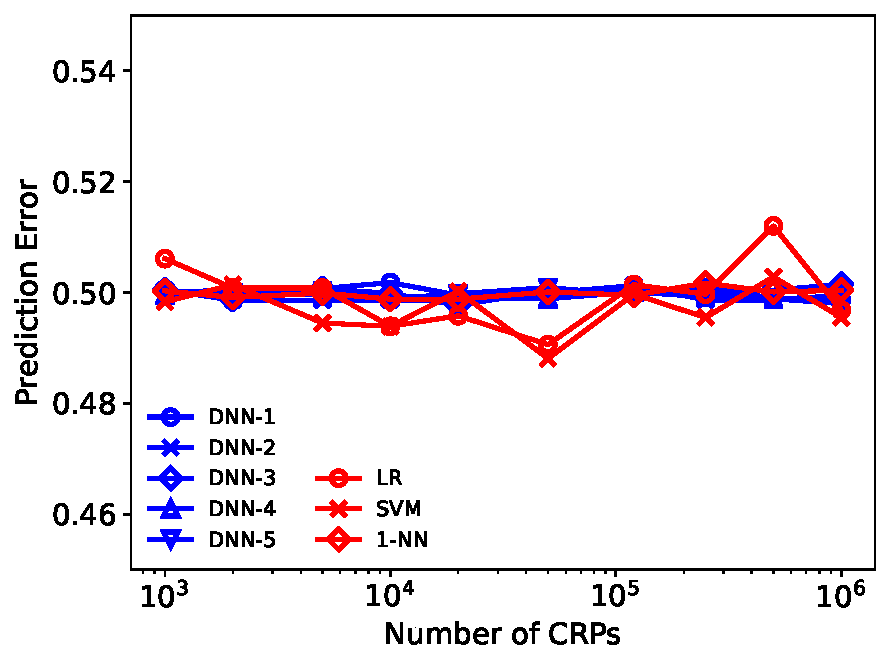
\includegraphics[width=0.5\linewidth]{./figs/ml_attack_lattice_puf.pdf}}
%  \caption{(a) ML attacks: Lattice PUF remains resistant to all attacks (DNNs, LR, SVM,1-NN). DNN ultimately succeeds in modeling two other strong PUFs. (b) Lattice PUF is resistant to both traditional ML attacks and DNNs.}
%  \label{fig: lattice_puf_ml_attack_results} 
%\end{figure}

\begin{table}[t!]
\centering
	%\caption{Different DNN configurations in modeling attacks.}
	%\label{table:DNNSetting}
	\resizebox{\linewidth}{!}{
        \begin{tabular}{|c|c|c|c|c|c|}
        \hline
        \textbf{Setup} & \begin{tabular}[c]{@{}l@{}}\textbf{Hidden}\\ \textbf{Layers}\end{tabular} & \begin{tabular}[c]{@{}c@{}}\textbf{Neurons}\\ \textbf{per Layer}\end{tabular} & \begin{tabular}[c]{@{}c@{}}\textbf{Challenge} \\ \textbf{Distribution}\end{tabular} & \begin{tabular}[c]{@{}c@{}}\textbf{Input} \\ \textbf{Format}\end{tabular} & \begin{tabular}[c]{@{}c@{}}\textbf{Prediction}\\ \textbf{Error}\end{tabular} \\ \hline
        DNN-1     & 4                                                       & 100                                                         & PRNG                                                              & Binary                                                  & 49.86\%                                                       \\ \hline
        DNN-2     & 4                                                       & 100                                                         & PRNG                                                              & Real                                                    & 49.84\%                                                       \\ \hline
        DNN-3     & 4                                                       & 100                                                         & Ciphertext                                                        & Binary                                                  & 49.76\%                                                       \\ \hline
        DNN-4     & 6                                                       & 100                                                         & PRNG                                                              & Binary                                                  & 49.80\%                                                       \\ \hline
        DNN-5     & 4                                                       & 200                                                         & PRNG                                                              & Binary                                                  & 49.87\%                                                       \\ \hline
        DNN-6     & 12                                                       & 2000                                                         & PRNG                                                              & Binary                                                  &    49.95\%                                                    \\ \hline
        \end{tabular}
    }
    \vspace{1em}
    \caption{Different DNN configurations in modeling attacks.}
    \label{table:DNNSetting}
    \vspace{-2em}
\end{table}

%DNNs are more powerful in binary classification. DNNs contain multiple hidden layers which enable superior modeling expressiveness compared to 1-NNs \cite{goodfellow2016deep}. Notably, recent successful DNN-based attacks have been demonstrated on published strong PUFs, including XOR APUFs and IPUFs \cite{DBLP:journals/iacr/SantikellurBC19}. Our baseline DNN experiment (DNN-1) adopts the same network parameters as in \cite{DBLP:journals/iacr/SantikellurBC19}.  The network has 4 hidden layers, each containing 100 neurons. It uses ReLU as the non-linear operator. 

DNN is a class of ML algorithms often highly effective in classification tasks. 
Its superior performance against 1-NNs is enabled by the expressiveness of multiple hidden neuron layers. Notably, recent successful DNN-based attacks have been demonstrated on strong PUFs, such as IPUFs \cite{DBLP:journals/iacr/SantikellurBC19},  XOR APUFs \cite{DBLP:journals/iacr/SantikellurBC19} and XOR BR PUFs \cite{dnn_xor_br_puf}. We select the DNN parameters in \cite{DBLP:journals/iacr/SantikellurBC19} as our baseline configuration (DNN-1): the number of hidden layers is 4, the number of neurons per layer is 100, and the activation function is ReLU.  

%Besides the parameters used in the baseline experiment, we varied network architectures, hyper-parameters, and numeric representations in the attack, as listed in Table \ref{table:DNNSetting}. 
%DNN-2 treats input as 161 integer numbers from 0 to 255, instead of 1288 binary bits.
%DNN-3 is different from the baseline version in its CRP generation strategy (see more below).
%DNN-4 and DNN-5 add more hidden layers and more neurons per hidden layer respectively, compared to the baseline DNN-1.

We explored multiple DNN configurations beyond the baseline experiment, Table \ref{table:DNNSetting}. The input to DNN-2 concatenates 161 8-bit integers. The input to DNN-3 follows a different challenge distribution. DNN-4 has an increased number of hidden layers and DNN-5 has an increased number of neurons within each layer. DNN-6 follows the configuration of a recent attack on XOR BR PUFs \cite{dnn_xor_br_puf}, and has a much larger number of both hidden layers and neurons per layer.

%Figure \ref{fig:ml_attack_2} shows the results of the empirical attacks based on the above ML algorithms. The figure shows the prediction error of lattice PUF in response to these attacks with training set size ranging from $1000$ to $1$ million and test set of size $200$K. The Adam optimizer \cite{kingma2014adam} terminates after 200 epochs, and results in a prediction error of $49.86\%$, barely better than a random guess. \emph{The results show that the prediction error of lattice PUF remains flat for all attempted attacks: across the range of attacks and CRP training set sizes, there is no measurable deviation of the error from 0.5.} In contrast, a DNN (with a configuration corresponding to DNN-1) achieves less than $2\%$ prediction error for both 4-XOR APUF and (4, 4)-IPUF.

The lattice PUF again demonstrates near perfect empirical ML resistance, Figure \ref{fig:ml_attack_2}. The results are reported using a test set with 200K CRPs and the DNNs are trained with the Adam optimizer running for 200 epochs. Regardless of the algorithms and the number of training CRPs used in the attack, the prediction error remains close to 0.5, which is equivalent to a random coin-flip. However, the two other strong PUFs can be successfully modelled by DNNs, with a prediction error smaller than 2\%.

%It is important to note that the experiments also show that the use of distributional relaxation of space-efficient LWE (described in Section \ref{sec:lfsr}) does not hinder empirical ML resistance of lattice PUF. In Table 1, all design/attack combinations except for DNN-3 are based on the compact (relaxation-based) design in which CRPs are generated via a PRNG. Finally, we show a detailed view of ML attack results on lattice PUF in Figure \ref{fig:ml_attack_3} by zooming in Figure \ref{fig:ml_attack_2}. While run-to-run variations of the training optimizer are observable, the prediction error remains close to $50\%$.

The results also validate the challenge compression technique demonstrated in Section \ref{sec:lfsr}. The DNN-1, DNN-2, DNN-4, DNN-5, and DNN-6 adopt challenges produced by the PRNG, but still show a prediction error close to 0.5. Figure \ref{fig:ml_attack_3} shows a zoomed view of DNN attack results on lattice PUF.

\subsection{Hardware Implementation Results}
\label{sec:hardware_results}

In this section, we show the hardware implementation details of lattice PUF. We synthesize, configure and test the entire design on a low-end XC6SLX45 FPGA device of Xilinx Spartan-6 family.  

We adopt the homogeneous error assumption regarding the RFE design. This means all cells are assumed to have the same BER \cite{bosch2008efficient}.
The BER of different POKs varies from $0.1\%$ \cite{karpinskyy20168} to $15\%$ \cite{maes2009soft}.
We configure BER = $1\%$, BER = $5\%$, BER = $10\%$ and BER = $15\%$ to investigate design trade-offs in RFE and POK, and finally configure the BER of SRAM POK in our design to be $5\%$. The RFE targets a $10^{-6}$ failure rate in reconstruction of $1280$ key bits. 
As described in Section \ref{sec:design}, the overall lattice PUF response BER can achieve the desired value with such a low key reconstruction failure rate.
Our error-correcting code (ECC) concatenates an inner code and an outer code. The inner code adopts repetition code and the outer code adopts shortened BCH code. Concatenated ECCs usually have shorter code length and lower hardware cost, compared to single codes \cite{bosch2008efficient}.
As described in Section \ref{sec:design}, the RFE scheme needs only lightweight encoder implementation on the device side. 
Table \ref{table:ecc} and \ref{table:hardware_fe} show the parameters and hardware utilization of ECCs with different configurations for BER.
A $5\%$ BER value requires $6.36K$ SRAM cells in order to reconstruct the $1280$-bit secret value $\mathbf{s}$ with a failure rate of $10^{-6}$.
The RFE encoder design requires $26$ slices. 
We adopt the SRAM-based design of \cite{aysu2015end} to implement the TRNG. The advantage is that the SRAM cells used to generate $\mathbf{s}$ can be reused for the SRAM-TRNG design. 
We adopt the 8-fold XORing of SRAM bits in \cite{aysu2015end} and therefore need $10.06K$ (i.e. $3.7K$ additional) SRAM cells. 
The 8-fold XORing logic design requires $1$ slice. 
Then, for the $5\%$ raw BER, the RFE design requires $27$ slices in total. 


%\begin{table}[t!]
%\centering
%\caption{Latency of different lattice PUF designs for 128-bit response generation [$\mu$s]. $P_1$ denotes number of LFSR-LWEDec data-paths; $P_2$ denotes number of LFSR output bits.} 
%\label{table:latency_par}
%\begin{tabular}{cccccccc}
%\hline
%\multicolumn{1}{|l|}{}            & \multicolumn{7}{c|}{\textbf{$\mathbf{P_2}$}}                                                                                                                                                                                                                 \\ \hline
%\multicolumn{1}{|c|}{\textbf{$\mathbf{P_1}$}} & \multicolumn{1}{c|}{\textbf{1}} & \multicolumn{1}{c|}{\textbf{4}} & \multicolumn{1}{c|}{\textbf{8}} & \multicolumn{1}{c|}{\textbf{16}} & \multicolumn{1}{c|}{\textbf{32}} & \multicolumn{1}{l|}{\textbf{64}} & \multicolumn{1}{l|}{\textbf{128}} \\ \hline
%\multicolumn{1}{|c|}{\textbf{1}}  & \multicolumn{1}{c|}{5632}       & \multicolumn{1}{c|}{1843}       & \multicolumn{1}{c|}{1229}       & \multicolumn{1}{c|}{614}         & \multicolumn{1}{c|}{307}         & \multicolumn{1}{c|}{154}         & \multicolumn{1}{c|}{77}           \\ \hline
%\multicolumn{1}{|c|}{\textbf{2}}  & \multicolumn{1}{c|}{2765}       & \multicolumn{1}{c|}{922}        & \multicolumn{1}{c|}{614}        & \multicolumn{1}{c|}{307}         & \multicolumn{1}{c|}{154}         & \multicolumn{1}{c|}{77}          & \multicolumn{1}{c|}{38}           \\ \hline
%\multicolumn{1}{|c|}{\textbf{4}}  & \multicolumn{1}{c|}{1382}       & \multicolumn{1}{c|}{461}        & \multicolumn{1}{c|}{307}        & \multicolumn{1}{c|}{154}         & \multicolumn{1}{c|}{77}          & \multicolumn{1}{c|}{38}          & \multicolumn{1}{c|}{NA}           \\ \hline
%\multicolumn{1}{|c|}{\textbf{8}}  & \multicolumn{1}{c|}{691}        & \multicolumn{1}{c|}{230}        & \multicolumn{1}{c|}{154}        & \multicolumn{1}{c|}{77}          & \multicolumn{1}{c|}{38}          & \multicolumn{1}{c|}{NA}          & \multicolumn{1}{c|}{NA}           \\ \hline
%\multicolumn{1}{l}{}              & \multicolumn{1}{l}{}            & \multicolumn{1}{l}{}            & \multicolumn{1}{l}{}            & \multicolumn{1}{l}{}             & \multicolumn{1}{l}{}             & \multicolumn{1}{l}{}             & \multicolumn{1}{l}{}              \\
%\multicolumn{1}{l}{}              & \multicolumn{1}{l}{}            & \multicolumn{1}{l}{}            & \multicolumn{1}{l}{}            & \multicolumn{1}{l}{}             & \multicolumn{1}{l}{}             & \multicolumn{1}{l}{}             & \multicolumn{1}{l}{}             
%\end{tabular}
%\end{table}
                          

%\begin{table}[t!]
%\centering
%\caption{Hardware utilization of different lattice PUF designs [slices]. $P_1$ denotes number of LFSR-LWEDec data-paths; $P_2$ denotes number of LFSR output bits.}
%\label{table:hwslices_par}
%\begin{tabular}{cccccccc}
%\hline
%\multicolumn{1}{|l|}{}            & \multicolumn{7}{c|}{\textbf{$\mathbf{P_2}$}}                                                                                                                                                                                                                 \\ \hline
%\multicolumn{1}{|c|}{\textbf{$\mathbf{P_1}$}} & \multicolumn{1}{c|}{\textbf{1}} & \multicolumn{1}{c|}{\textbf{4}} & \multicolumn{1}{c|}{\textbf{8}} & \multicolumn{1}{c|}{\textbf{16}} & \multicolumn{1}{c|}{\textbf{32}} & \multicolumn{1}{l|}{\textbf{64}} & \multicolumn{1}{l|}{\textbf{128}} \\ \hline
%\multicolumn{1}{|c|}{\textbf{1}}  & \multicolumn{1}{c|}{45}         & \multicolumn{1}{c|}{123}        & \multicolumn{1}{c|}{124}        & \multicolumn{1}{c|}{137}         & \multicolumn{1}{c|}{150}         & \multicolumn{1}{c|}{178}         & \multicolumn{1}{c|}{287}          \\ \hline
%\multicolumn{1}{|c|}{\textbf{2}}  & \multicolumn{1}{c|}{249}        & \multicolumn{1}{c|}{298}        & \multicolumn{1}{c|}{301}        & \multicolumn{1}{c|}{320}         & \multicolumn{1}{c|}{373}         & \multicolumn{1}{c|}{362}         & \multicolumn{1}{c|}{465}          \\ \hline
%\multicolumn{1}{|c|}{\textbf{4}}  & \multicolumn{1}{c|}{348}        & \multicolumn{1}{c|}{463}        & \multicolumn{1}{c|}{463}        & \multicolumn{1}{c|}{546}         & \multicolumn{1}{c|}{629}         & \multicolumn{1}{c|}{631}         & \multicolumn{1}{c|}{NA}           \\ \hline
%\multicolumn{1}{|c|}{\textbf{8}}  & \multicolumn{1}{c|}{561}        & \multicolumn{1}{c|}{834}        & \multicolumn{1}{c|}{847}        & \multicolumn{1}{c|}{920}         & \multicolumn{1}{c|}{1015}        & \multicolumn{1}{c|}{NA}          & \multicolumn{1}{c|}{NA}           \\ \hline
%\multicolumn{1}{l}{}              & \multicolumn{1}{l}{}            & \multicolumn{1}{l}{}            & \multicolumn{1}{l}{}            & \multicolumn{1}{l}{}             & \multicolumn{1}{l}{}             & \multicolumn{1}{l}{}             & \multicolumn{1}{l}{}              \\
%\multicolumn{1}{l}{}              & \multicolumn{1}{l}{}            & \multicolumn{1}{l}{}            & \multicolumn{1}{l}{}            & \multicolumn{1}{l}{}             & \multicolumn{1}{l}{}             & \multicolumn{1}{l}{}             & \multicolumn{1}{l}{}             
%\end{tabular}
%\end{table}


% \begin{figure}[t!]
% \centering
% 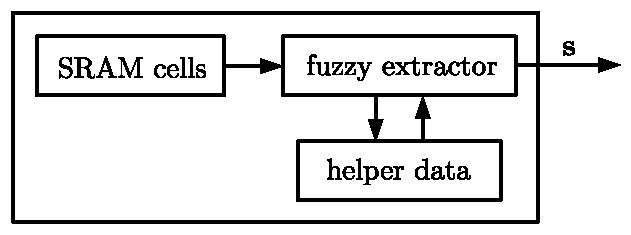
\includegraphics[width = 0.75\linewidth]{./figs/pok.pdf}
% \caption{POK uses an FE to ensure stability of the secret seed.}
% \label{fig:pok}
% \end{figure}

%We now present the details of implementing the lattice PUF, as shown in Figure \ref{fig:fpga_impl}. 
%In this section, we show the hardware implementation details of lattice PUF. The entire design, except for the raw (uninitialized) SRAM cells, was synthesized, configured, and tested on a Xilinx Spartan-6 FPGA (XC6SLX45), a low-end FPGA in 45nm technology.

%The cost of FE/RFE applies to all other strong PUF candidates (AES PUF or other controlled PUF).
%This is also cheaper than linear solver block used in the CFE-based strong PUF \cite{herder2017trapdoor,jin2017fpga} for key reconstruction, which requires $65,700$ LUTs and $16,425$ slices.

The lattice PUF (without RFE) takes a total of 45 slices on Spartan-6 FPGA. The LFSR and the controller occupies most of the slices. Table %\ref{table:fpga_utilization}
\ref{table:fpga_result}(a) shows the resources breakdown of each module. The decryption function of LWE (LWEDec) is implemented with MAC unit of 8 bits and a block for MAC result quantization, Figure \ref{fig:lwedec}.
RAM-based shift registers are used to implement the 256-bit LFSR. It takes $47\mu$s in total to generate a single PUF response bit under a clock running at 33.3MHz. 100 PUF response bits require about $4.4ms$ ($8\mu s + 100\times 44\mu s$) in total. Table %\ref{table:fpga_timing} 
\ref{table:fpga_result}(b) shows latency of each procedure to produce a PUF response.

\begin{table}[t!]
    %\caption{(a) Area consumption and (b) runtime of our reference lattice PUF implementation on Xilinx Spartan-6 FPGA.}
    %\label{table:fpga_result}
    \centering
    \def\arraystretch{1.1}
    \subfloat[]{
        \resizebox{0.45\linewidth}{!}{
            \begin{tabular}{|c|c|}
            \hline
            \textbf{Module}         & \textbf{Size [slices]} \\ \hline
            LFSR                    & 27            \\ \hline
            LWEDec                  & 2             \\ \hline
            Controller              & 16            \\ \hline
            \textit{Total}          & 45            \\ \hline
            \end{tabular}
            %\label{table:fpga_utilization}
        }
    }
    \hspace{1em}
    \subfloat[]{
        \resizebox{0.75\linewidth}{!}{
            \begin{tabular}{|c|c|}
            \hline
            \textbf{Step}                               & \textbf{Time [$\mu$s]} \\ \hline
            Seed $\text{seed}_{\mathbf{a}'}||t$ load for LFSR    & 8             \\ \hline
            1-bit decryption from LWEDec                  & 44            \\ \hline
            \textit{Total} @ 33 \textit{MHz}            & 52            \\ \hline
            \end{tabular}
            %\label{table:fpga_timing}
        }
    }
    \vspace{1em}
    \caption{(a) Area consumption and (b) runtime of our reference lattice PUF implementation on Xilinx Spartan-6 FPGA.}
    \label{table:fpga_result}
\end{table}

We now explore the design space of our proposed lattice PUF, starting with the resource-efficient design. We adopt the parallelization strategies proposed in Section \ref{sec: lpuf_par} and implement designs with different levels of parallelism. The latency and hardware utilization of the designs are summarized in Table \ref{table:latency_par} and \ref{table:hwslices_par}. Fig. \ref{fig:design_space_latency} and Fig. \ref{fig:design_space_hw} visualize the influence of $P_1$ and $P_2$ on latency and hardware cost. Similar to Table %\ref{table:fpga_utilization}
\ref{table:fpga_result}(a), we report the sum of slice utilization of LFSR, LWEDec and Controller modules. The maximum value of $P_2$ is $128$ due to the constraint of LFSR generator polynomial. Table entries with NA indicate the corresponding design requires more multipliers than the available DSP slices on the device. We observe that the parallelized design leads to a steady reduction in latency, at the cost of increased hardware utilization. We achieve a 148X reduction in latency in the most latency-optimized design, with a 10X increase in hardware utilization. %While both parallelization strategies demonstrate effectiveness in latency reduction, they have different efficiency in hardware utilization. 
In addition, we observe the MAC unit parallelization strategy has better hardware efficiency compared to LFSR-LWEDec datapath parallelization strategy. To achieve the same latency reduction, the design which prioritizes MAC unit parallelization requires fewer slices. For instance, to achieve the optimal $38 \mu$s latency, the design with $(P_1, P_2) = (2, 128)$ only requires $465$ slices, while the design with $(P_1, P_2) = (8, 32)$ requires $1,015$ slices. This validates our optimal strategy demonstrated in Section \ref{sec: lpuf_par}. %This seems to indicate the LFSR unrolling is always a better strategy for latency optimization. However, in reality, the LFSR cannot be unrolled by unlimited times while keeping the equivalent functionality. The LFSR generator polynomial limits the maximum unrolling times. For instance, if the 256-bit LFSR takes the XOR result of $X_{255}$, $X_{253}$, $X_{250}$ and $X_{7}$ as the feedback bit, the LFSR cannot be unrolled by over 8 times with the technique presented in Section \ref{sec: lpuf_par}, since the LSB $X_{0}$ is only 8 bits away from $X_{7}$. Therefore, in practice, the optimal strategy is to first seek parallelization via LFSR unrolling, and then parallelize the LFSR-LWEDec data-path to achieve further latency optimization once the unrolling of LFSR reaches the limit.

\begin{table}[t!]
\centering
	%\caption{Comparison of hardware utilization of various strong PUFs.}
	\vspace{-0.5em}
	%\label{table:hardware_puf}
	\def\arraystretch{1.1}
	\resizebox{\linewidth}{!}{
        \begin{tabular}{|c|c|c|c|c|c|c|}
        \hline
        \textbf{Design} & \textbf{Platform} & \begin{tabular}[c]{@{}c@{}}\textbf{PUF Logic}\\ \textbf{[Slices]}\end{tabular} & \begin{tabular}[c]{@{}c@{}@{}@{}}\textbf{Error-}\\ \textbf{Correction}\\\textbf{Code}\\ \textbf{[Slices]}\end{tabular} & \begin{tabular}[c]{@{}c@{}}\textbf{POK}\\ \textbf{[Bits]}\end{tabular} & \begin{tabular}[c]{@{}c@{}}\textbf{Response}\\ \textbf{[Bits]}\end{tabular} & \begin{tabular}[c]{@{}c@{}}\textbf{Latency}\\ \textbf{[$\mu$s]}\end{tabular} \\\hline
        POK+AES \cite{bhargava2014efficient} & Spartan 6 & 80 & 27 & 612 & 128 & 2.2\\ \hline
        Controlled PUF \cite{gassend2008controlled} & Spartan 6 & 127 & 27 & 612 & 256 & 19.1\\ \hline
        \begin{tabular}[c]{@{}c@{}}CFE-based PUF\\ \cite{herder2017trapdoor,jin2017fpga}\end{tabular} & Zynq-7000 & 9,225 & 0 & 450\tablefootnote{The POK is based on RO PUF and assumes a different BER.} & 256 & 658\tablefootnote{Zynq-7000 device typically runs faster than Spartan-6 device.}\\ \hline
        \begin{tabular}[c]{@{}c@{}}Lattice PUF\\ (resource-efficient)\end{tabular} & Spartan 6 & 45 & 26 & 6,360 & 128 & 5,632\\ \hline
        \begin{tabular}[c]{@{}c@{}}Lattice PUF\\ (latency-optimized)\end{tabular} & Spartan 6 & 465 & 26 & 6,360 & 128 & 38\\ \hline
        \end{tabular}
    }
    \vspace{1em}
    \caption{Comparison of hardware utilization of various strong PUFs.}
    \label{table:hardware_puf}
\end{table}

\begin{table}[t!]
    \centering
	%\caption{Configuration of concatenated ECCs.}
	%\vspace{-0.5em}
	%\label{table:ecc}
	\def\arraystretch{1.1}
	\resizebox{0.9\linewidth}{!}{
        \begin{tabular}{|c|c|c|c|c|c|}
        \hline
        \multirow{2}{*}{\begin{tabular}[c]{@{}c@{}}\textbf{Raw BER}\\  \textbf{(\%)}\end{tabular}} & \multicolumn{2}{c|}{\textbf{Error-Correcting Code}}                                 & \multirow{2}{*}{\textbf{Raw POKs}}  \\ \cline{2-3} 
                                                                                 & Outer code   & Inner code & \\ \hline
        1                                                                        & {[}236, 128, 14{]}  & N/A            & 2,360  \\ \hline
        5                                                                        & {[}212, 128, 11{]} & {[}3, 1, 1{]}  & 6,360  \\ \hline
        10                                                                       & {[}220, 128, 12{]} & {[}5, 1, 2{]}  & 11,000  \\ \hline
        15                                                                       & {[}244, 128, 15{]} & {[}7, 1, 3{]}  & 17,080   \\ \hline
        \end{tabular}
    }
    \vspace{1em}
    \caption{Configuration of concatenated ECCs.}
    \label{table:ecc}
\end{table}

\begin{table*}[t!]
    \centering
    %\caption{Hardware utilization in ECC encoder design on Spartan 6 FPGA.}
    %\label{table:hardware_fe}
        \begin{tabular}{|c|c|c|c|c|c|c|c|c|c|}
        \hline
        \multirow{2}{*}{\begin{tabular}[c]{@{}c@{}}\textbf{Raw BER}\\  \textbf{(\%)}\end{tabular}} & \multicolumn{3}{c|}{\textbf{Outer Code}} & \multicolumn{3}{c|}{\textbf{Inner Code}} & \multicolumn{3}{c|}{\textbf{Total}} \\ \cline{2-10} 
                               & Reg      & LUT      & Slice     & Reg      & LUT      & Slice     & Reg    & LUT    & Slice    \\ \hline
        1                      & 112      & 93       & 30        & 0        & 0        & 0         & 112    & 93     & 30       \\ \hline
        5                      & 96       & 78       & 25        & 1        & 1        & 1         & 97     & 79     & 26       \\ \hline
        10                     & 96       & 83       & 28        & 1        & 1        & 1         & 97     & 84     & 29       \\ \hline
        15                     & 120      & 105      & 35        & 1        & 1        & 1         & 121    & 106    & 36       \\ \hline
        \end{tabular}
        \vspace{1em}
        \caption{Hardware utilization in ECC encoder design on Spartan 6 FPGA.}
    \label{table:hardware_fe}
\end{table*}

\begin{table}[t!]
\centering
%\caption{Latency of different lattice PUF designs for 128-bit response generation [$\mu$s]. $P_1$ denotes number of LFSR-LWEDec data-paths; $P_2$ denotes number of LFSR output bits.}
%\label{table:latency_par}
\begin{tabular}{|c|*{7}{c|}}\hline
\backslashbox{\textbf{$\mathbf{P_1}$}}{\textbf{$\mathbf{P_2}$}}
&\makebox{\textbf{1}}&\makebox{\textbf{4}}&\makebox{\textbf{8}}
&\makebox{\textbf{16}}&\makebox{\textbf{32}}&\makebox{\textbf{64}}&\makebox{\textbf{128}}\\\hline
\textbf{1} & 5,632 & 1,843 & 1,229 & 614 & 307 & 154 & 77\\\hline
\textbf{2} & 2,765 & 922 & 614 & 307 & 154 & 77 & 38\\\hline
\textbf{4} & 1,382 & 461 & 307 & 154 & 77 & 38 & NA\\\hline
\textbf{8} & 691 & 230 & 154 & 77 & 38 & NA & NA\\\hline
\end{tabular}
\vspace{1em}
\caption{Latency of different lattice PUF designs for 128-bit response generation [$\mu$s]. $P_1$ denotes number of LFSR-LWEDec data-paths; $P_2$ denotes number of LFSR output bits.}
\label{table:latency_par}
\end{table}

\begin{table}[t!]
\centering
%\caption{Hardware utilization of different lattice PUF designs [slices]. $P_1$ denotes number of LFSR-LWEDec data-paths; $P_2$ denotes number of LFSR output bits.}
%\label{table:hwslices_par}
\begin{tabular}{|c|*{7}{c|}}\hline
\backslashbox{\textbf{$\mathbf{P_1}$}}{\textbf{$\mathbf{P_2}$}}
&\makebox{\textbf{1}}&\makebox{\textbf{4}}&\makebox{\textbf{8}}
&\makebox{\textbf{16}}&\makebox{\textbf{32}}&\makebox{\textbf{64}}&\makebox{\textbf{128}}\\\hline
\textbf{1} & 45 & 123 & 124 & 137 & 150 & 178 & 287\\\hline
\textbf{2} & 249 & 298 & 301 & 320 & 373 & 362 & 465\\\hline
\textbf{4} & 348 & 463 & 463 & 546 & 629 & 631 & NA\\\hline
\textbf{8} & 561 & 834 & 847 & 920 & 1015 & NA & NA\\\hline
\end{tabular}
\vspace{1em}
\caption{Hardware utilization of different lattice PUF designs [slices]. $P_1$ denotes number of LFSR-LWEDec data-paths; $P_2$ denotes number of LFSR output bits.}
\label{table:hwslices_par}
\end{table}



%\begin{figure}[t!]
%\centering
%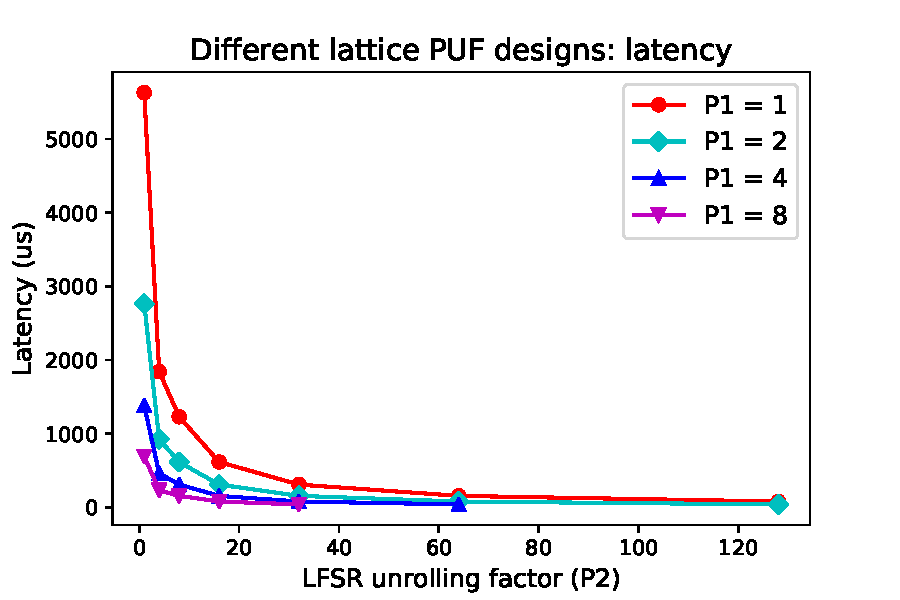
\includegraphics[width = 0.8\linewidth]{./figs/design_space_latency.pdf}
%\caption{Increasing $P_1$ and $P_2$ leads to steady reduction in latency.}
%\label{fig:design_space_latency}
%\end{figure}

%\begin{figure}[t!]
%\centering
%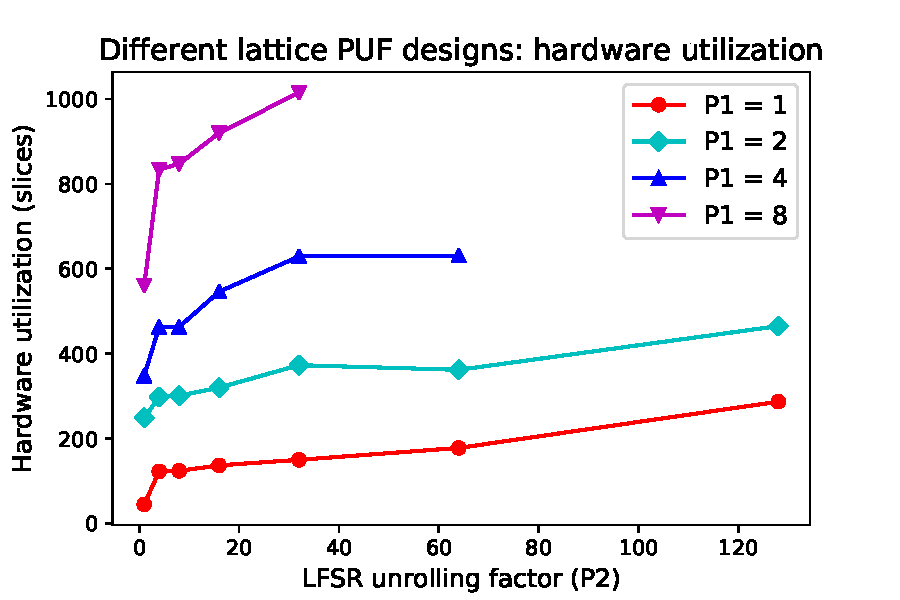
\includegraphics[width = 0.8\linewidth]{./figs/design_space_hw.pdf}
%\caption{Increasing $P_2$ is more hardware efficient than increasing $P_1$, but maximum $P_2$ is limited by the LFSR generator polynomial. The optimal strategy is to increase $P_2$ first to achieve latency goal. If $P_2$ reaches the limit and more aggressive latency reduction is required, increase $P_1$.}
%\label{fig:design_space_hw}
%\end{figure}

We finally compare the hardware utilization and latency of lattice PUF designs to several published strong PUF designs \cite{bhargava2014efficient, gassend2008controlled, jin2017fpga} who also have ML resistance in Table \ref{table:hardware_puf}. 
As mentioned in Section \ref{sec:intro}, there are two different categories of ML resistance among those listed PUFs. 
ML resistance of the AES-based PUF and the controlled PUF can be reduced to the security of the deployed primitives. 
In contrast, the theoretical ML resistance of the CFE-based strong PUF and our lattice PUF can be reduced to the hardness of fundamental math problems, like LPN and LWE.
The original proposal of the AES-based strong PUF \cite{bhargava2014efficient} is an ASIC implementation. 
Here, to estimate the AES implementation cost in FPGA, we adopt results in \cite{chu2012low}.
Note that the original proposal of \cite{bhargava2014efficient} does not use FE-based error correction: it uses dark bit masking to guarantee reliability. 
To estimate the cost of its error correction on an FPGA implementation, we use the RFE encoder design for a 128-bit key reconstruction with a $5\%$ raw BER and $10^{-6}$ failure rate, similar to the ECC design for the lattice PUF. The estimated number of raw POK bits are derived using these parameters.
Similarly, to calculate hash function hardware utilization in the controlled PUF \cite{gassend2008controlled}, the FPGA implementation results of SHA-3 in \cite{sha3_finalist} is used. 
No design details of the error correction and the POK are given in the proposal of controlled PUF \cite{gassend2008controlled}. We follow the same assumption as for the AES PUF for estimation.
\cite{jin2017fpga} reports the hardware utilization results of the computational FE (CFE) based strong PUF on FPGA in the LUT numbers.
By utilizing \cite{xilinx:ds190}, we convert the LUT numbers to the slice numbers. 
The CFE-based strong PUF does not use a conventional FE-based error correction so its ECC cost is 0.

Table \ref{table:hardware_puf} shows that the resource-efficient version of the lattice PUF achieves the smallest slice number among all strong PUF designs with ML resistance.
From the latency perspective, the AES-based PUF and the controlled PUF run faster than the CFE-based PUF and our lattice PUF. This is primarily due to the fundamental algorithmic difference of the LWE problem and the established cryptographic primitives. The LWE problem requires sequential MACs on the elements of long vectors and produces a single output bit per execution, while AES finishes within a relatively small number of rounds and has a much larger output size.
Compared to the CFE-based strong PUF whose ML resistance can also be reduced to the hardness of a fundamental math problem, the resource-efficient lattice PUF achieves a 205X area reduction, and the latency-optimized version achieves a 16X latency improvement together with a 19X area reduction.
%Recall that the ML resistance of the CFE-based strong PUF and our lattice PUF can be reduced to the hardness of fundamental math problems while strong PUFs based on AES or hash functions can 
%We achieve a great reduction in area compared to the CFE-based strong PUF \cite{herder2017trapdoor, jin2017fpga}, which gives theoretical ML-resistance similarly. 
%\textcolor{red}{In the performance-critical scenario, our design produces response bits faster than the CFE-based PUF \cite{herder2017trapdoor, jin2017fpga}, but slower than the AES PUF and the controlled PUF. This is primarily due to the fundamental algorithmic difference of the LWE problem and the established cryptographic primitives. The LWE problem requires sequential MACs on the elements of long vectors and produces a single output bit per execution, while AES finishes within a relatively small number of rounds and has a much larger output size.} %(We note that it is possible to further reduce latency of lattice PUF following our parallelization strategy, if implementing multipliers utilizing non-DSP slices. The cost will be significantly increased hardware utilization. We plan to investigate lattice PUF architectures which allows efficient further improvements in latency for future work.)} 
%We find that the implementation cost of the lattice PUF (without FE) is cheaper than that of AES on POK, controlled PUF, and CFE-based PUF.

%\textcolor{red}{Since the lattice PUF fundamentally builds upon a POK and an LWE decryption function, one natural question is if the POK can be replaced with a secret key programmed directly in non volatile memory. While this alternative primitive further reduces hardware cost, it compromises security that is otherwise provided by POK (PUF). The keys stored explicitly and permanently in memory can be easily exploited by physical access attacks \cite{semi_invasive_attacks}. In contrast, keys derived from PUFs only establish their values when evaluating the PUF. The nature of PUFs hide keys from physical access attacks since it explores intrinsic randomness of CMOS technology. Therefore, the lattice PUF primitive rather than the PUF-less alternative should be adopted for better security guarantees.}
%A lattice PUF is realized by two major components: a POK and an LWE decryption function. The POK is needed for silicon-intrinsic key generation, with all the well-known security benefits of PUF-based key generation. A simpler NVM-based key storage mechanism in place of the POK is an alternative approach that is cheaper but with reduced security against physical key-extraction attacks. In this case, the design described in the paper can be thought as a keyed LWE-based hash function with restricted inputs (which follow the ciphertext distribution).
%Note that there exists another such construction, namely, the LWE-based pseudorandom function \cite{brenner2014fpga}, which can even guarantee ML resistance without input restrictions.  In fact, its hardware implementation requires more logic slices.

\begin{figure}[t!]
\centering
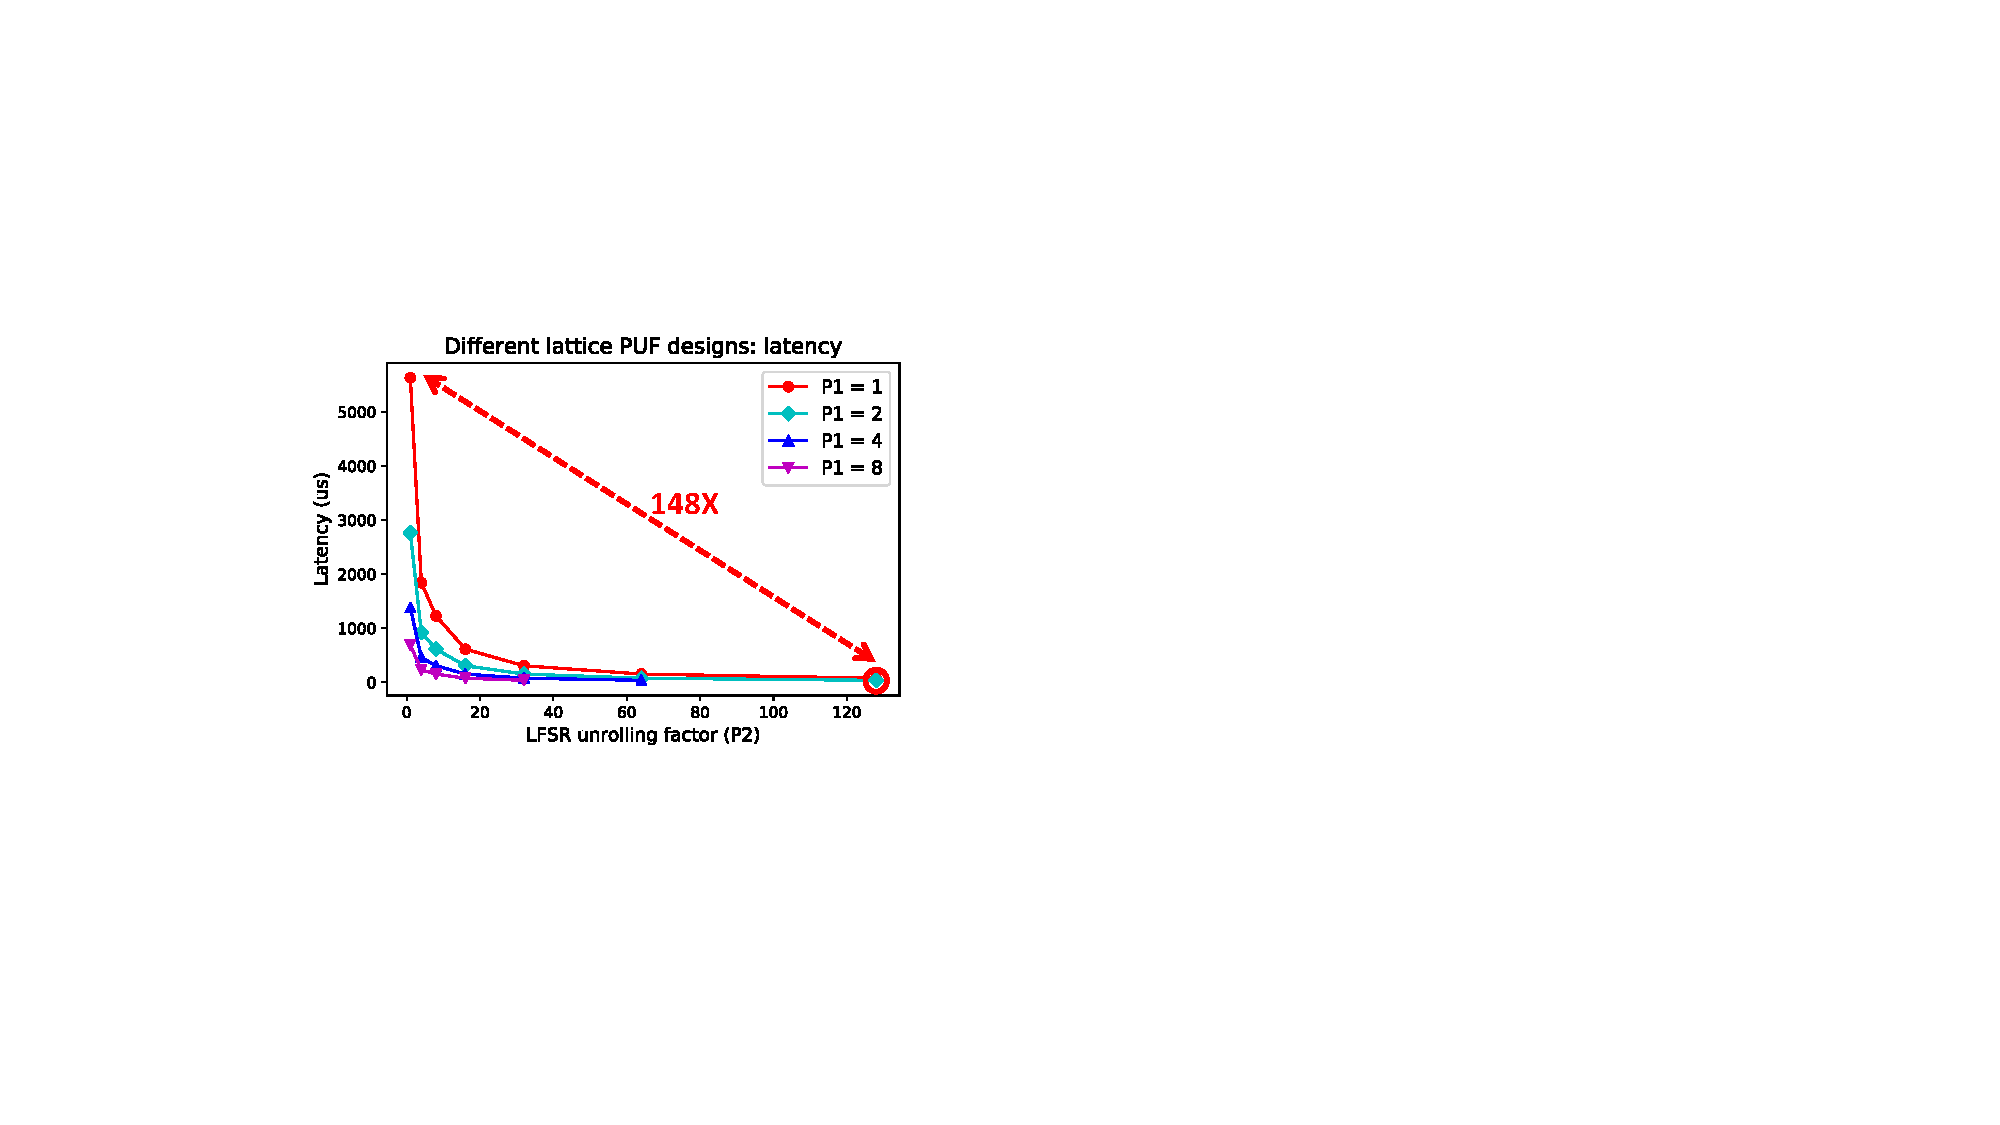
\includegraphics[width = 0.78\linewidth]{./figs/design_space_latency_annotated.pdf}
\caption{Increasing $P_1$ and $P_2$ leads to steady reduction in latency.}
\label{fig:design_space_latency}
\end{figure}

\begin{figure}[t!]
\centering
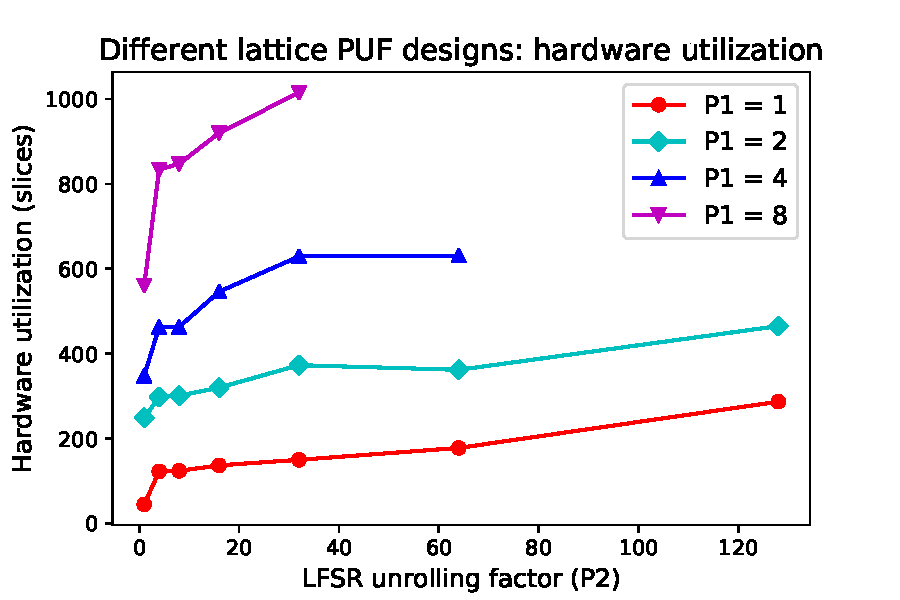
\includegraphics[width = 0.8\linewidth]{./figs/design_space_hw.pdf}
\caption{Increasing $P_2$ is more hardware efficient than increasing $P_1$, but maximum $P_2$ is limited by the LFSR generator polynomial. The optimal strategy is to increase $P_2$ first to achieve latency goal. If $P_2$ reaches the limit and more aggressive latency reduction is required, increase $P_1$.}
\label{fig:design_space_hw}
\end{figure}